%Include simulation results: both wave forms in time domain, and in frequency domain (apply FFT) (assignments 3 and 4 only).

Figure~\ref{fig:simulation:spectrum} shows the spectrum analysis of the input and the output files.
As you can see, the filter has a clear drop-off at around 3000Hz, which is what we are expecting.

\begin{figure}[H]
	\centering
	\begin{subfigure}[l]{0.7\textwidth}
		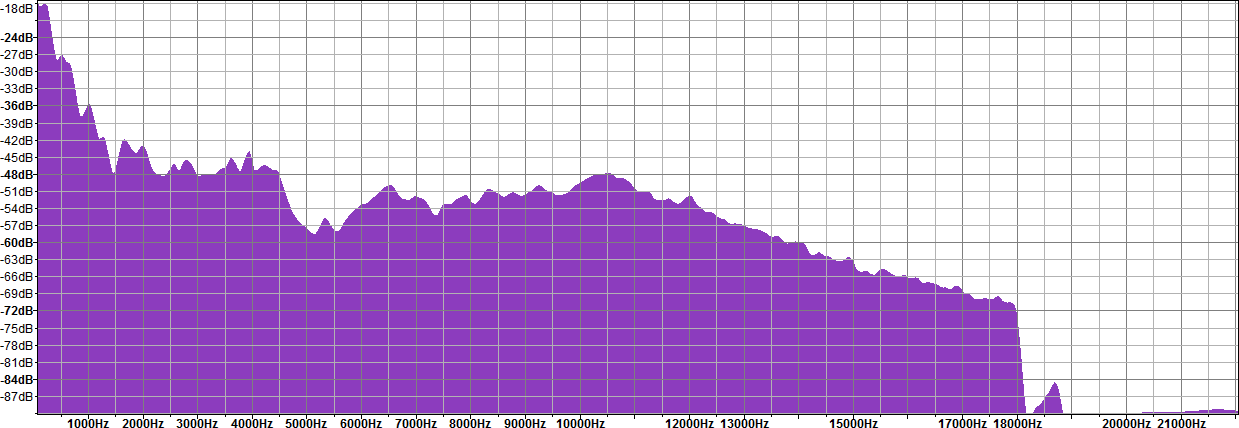
\includegraphics[width=\textwidth]{spectrum-before}
		\caption{Input}
		\label{fig:simulation:spectrum:before}
	\end{subfigure}

	\begin{subfigure}[l]{0.7\textwidth}
		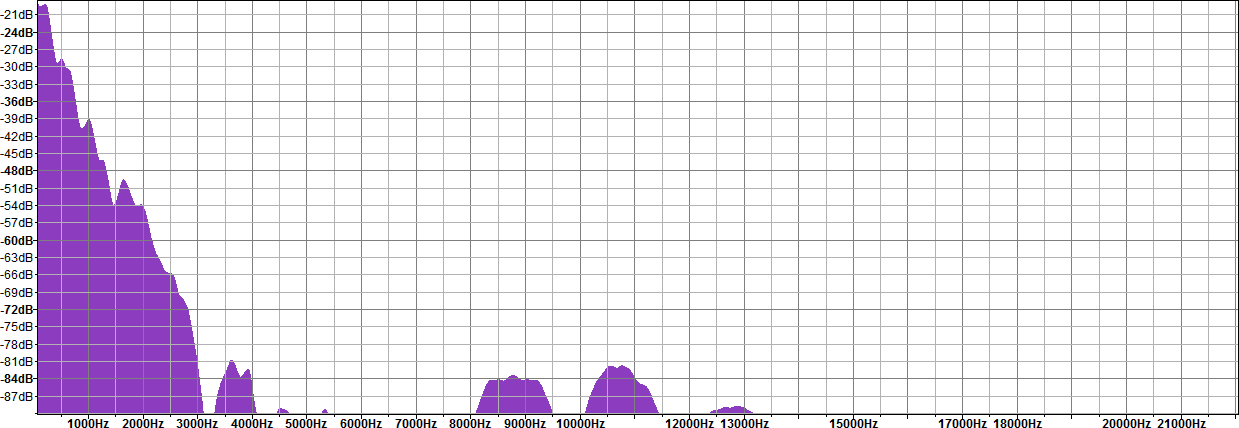
\includegraphics[width=\textwidth]{spectrum-after}
		\caption{Output}
		\label{fig:simulation:spectrum:after}
	\end{subfigure}

	\caption{Comparison of the audio spectrum before and after running the filter}
	\label{fig:simulation:spectrum}
\end{figure}

%TODO Matlab
